\documentclass[notitlepage]{report}
\usepackage{graphicx}
\usepackage[left=1in, right=1in, top=1in, bottom=1in]{geometry}
\usepackage{titling}
\usepackage{lipsum}
\pretitle{\begin{center}\Huge\bfseries}
\posttitle{\par\end{center}\vskip 0.5em}
\preauthor{\begin{center}\Large\ttfamily}
\postauthor{\end{center}}
%\predate{\par\large\centering}
%\postdate{\par}
\title{Higher-order Combinations of Existing Ideas}
\author{Us and others}
%\date{\today}
\date{}
\usepackage{color}
\begin{document}
\maketitle
\thispagestyle{empty}
Sir:\\

Co-citation, when two articles are cited by a third, represents the combination of two existing ideas into a third, and its frequency, which accumulates over time, represents the extent to which this idea is considered by the research community. Marshakova-Shaikevich and Small independently described co-citation in 1973, emphasizing its forward looking characteristics compared to bibliographic coupling, and co-citation measurements have since been extensively used in scientometrics.

From a sampling of the physics literature, Small reported 4 pairs of articles with a co-citation frequency of 49 and greater. The volume of scientific literature has grown considerably since; more co-cited pairs have been discovered; frequencies have increased; and the scale of studies has become larger. Improved bibliographies and modern computing tools have also rendered co-citation calculations relatively facile. 

Uzzi et al. reported a study on novelty in which they examined co-cited references from roughly 18 million articles. Devarakonda et al. reported that 1,309 of 33.6 million co-cited pairs derived from articles published in Scopus in the years 1985--1995 had co-citation frequencies of over 1,000. More recently, Zhao et al. have computed co-citation frequencies for 940 million co-cited article pairs from the same period and identified roughly 1,200 pairs with delayed kinetics analogous to Sleeping Beauty publications. 

A natural extension of co-citation theory is document coupling of a higher order, for example, triads, tetrads, and greater. Triads can be viewed as either the coming together of three previously independent ideas or the coalescence of three overlapping co-citations in the triad. Indeed, Small proposed a model of multiple citation in 1974 in which an example of tri-citations measured over a set of 6 publications were presented. In his report, Small used intersections of sets of citing papers to measure co-citation frequency, `If $A$ is the set of papers citing document $a$, and $B$ the set citing $b$,the frequency of co-citation of $a$ and $b$ is $n(A \cap B)$'.

An alternate way of looking at these patterns is to view any article $A$ that cites $n$ articles as comprising $n$ citations, $n\choose2$ co-citations, $n\choose3$ tri-citations etc. Calculating the frequencies of these combinations in a bibliography is relatively expensive, however. An article with either 25 or 50 cited references represents 300 or 1,225 co-citations respectively. The same article also consists of  2,300 or 19,600 tri-citations and  12,650 or  230,300 tetra-citations. For evena modestly sized collection of 2 million articles with an average of 30 references each, this could involve computing $8.12\times10^9$ tri-citations, $5.48\times10^{10}$ tetra-citations, or $2.85\times10^{11}$ penta-citations.  However, scalable and affordable computing today places measuring these higher order assemblies within reach of the scientometrist, and may open a new frontier for discovery

In an initial exploration of higher-order combinations, we have used a `brute force' approach to compute triad frequencies from an 11-year dataset of articles in the Scopus bibliography to identify 181 million triads that are tri-cited between 1 and 13,000 times. Much like citations and co-citations, the vast majority of tri-citations are of very low frequency. High frequency triplets naturally pique interest. 

We present an example with a tri-citation frequency of 13,000 (the highest that we observed) [need to add IDs] ; its component co-cited pairs have been co-cited 16,000, 25,000, and 52,000 times, and the individual articles in this triad have been cited 38,000, 72,000, and 75,000 times respectively (Figure 1). All three elements of the triad originate in density functional theory (DFT), a quantum mechanical (QM) theory that can be applied to a range of chemical problems. In this model two functionals of the electron density are needed (a functional can be described as a function of a function) to complete the model. One is the so-called Exchange functional (two electrons of the same spin cannot be at the same point in space) and the other is the Correlation functional (accounting for the correlated motion of electrons with the same spin). In the 1980’s a effort developed to build Exchange and Correlation functionals to allow for the practical application of DFT to chemical problems. This effort was pursued by a number of groups but the Becke group in its 1988 and 1993 papers developed an Exchange functional while Lee, Yang, and Parr developed a Correlation functional in their 1988 paper. 

Thus, this high frequency tri-citation could be explained by recognition of the two Becke papers providing the Exchange functional and the Lee-Yang-Parr with the Correlation functional. 
However, the first citation of this triplet likely arose because of a paper published by Stephens and co-workers in 1994 which blended these Exchange and Correlation functionals into a method called B3LYP (Becke-3 Exchange and Lee-Yang-Parr Correlation). The B3LYP method had a lot of advantages in terms of speed and accuracy for the study of organic molecules especially and was rapidly taken up by the computational chemistry and organic chemistry communities, which likely explains the high frequency of co-citation of Becke(1993) and LYP (1988). A concise summary of this major advance can be achieved by citing Becke (1988), LYP (1988) and Becke (1993). We note that Stephens, et al. (1994) as well as Vosko, Wilk and Nusair (1980) which helped form part of the LYP Correlation functional are also found in high frequency tri-citations (greater than 1,000) but are not as heavily tri-cited as Becke(1988), Lee, Yang, and Parr (1993), and Becke (1993). \emph{I am inclined to conclude that citations tell only part of the story}

\textcolor{blue}{
\emph{For KM. Apart from a general rule that co-citation frequencies are lower than citation frequencies, any thoughts on why Becke (1993) and LYP (1988) are cited so heavily on an individual basis?, Vosko, Wilk, and Nusair (1980) is not in Scopus and neither LYP (1993) nor Becke (1988) cite this paper. However  Becke 1993 cites J. P. Perdew, J. A. Chevary, S. H. Vosko, K. A. Jackson, M. R. Pederson, D. J. Singh, and C. Fiolhais, Phys. Rev. B 46, 6671 (1992) and Stephens et al. (1993) cites Vosko, Wilk, and Nusair (1980).}}  

\textcolor{blue}{
\emph{For KM. In order to correctly cite this method the three papers in question are appropriate along with the Stephens, et al. work as well as a paper by Vosko, Wilk and Nusair in 1980 which helped form part of the LYP Correlation functional. It is interesting to see if the paper of Stephens et al and Vosko et al form a co-citation pentuplet given their relationship in the form of the B3LYP DFT model. Stephens (1994), Becke (1993), LYP (1988), and Becke (1988) are quad-cited 2100 (2134) times. Stephens and any two of the Becke, Becke, LYP triplet are tri-cited between 280 and 6500 times- less than than 13,000 times Becke, Becke, and LYP are tri-cited). So the field seems to recognize Becke, Becke, LYP more than any other triple}}

\begin{figure}[h!]
\begin{center}
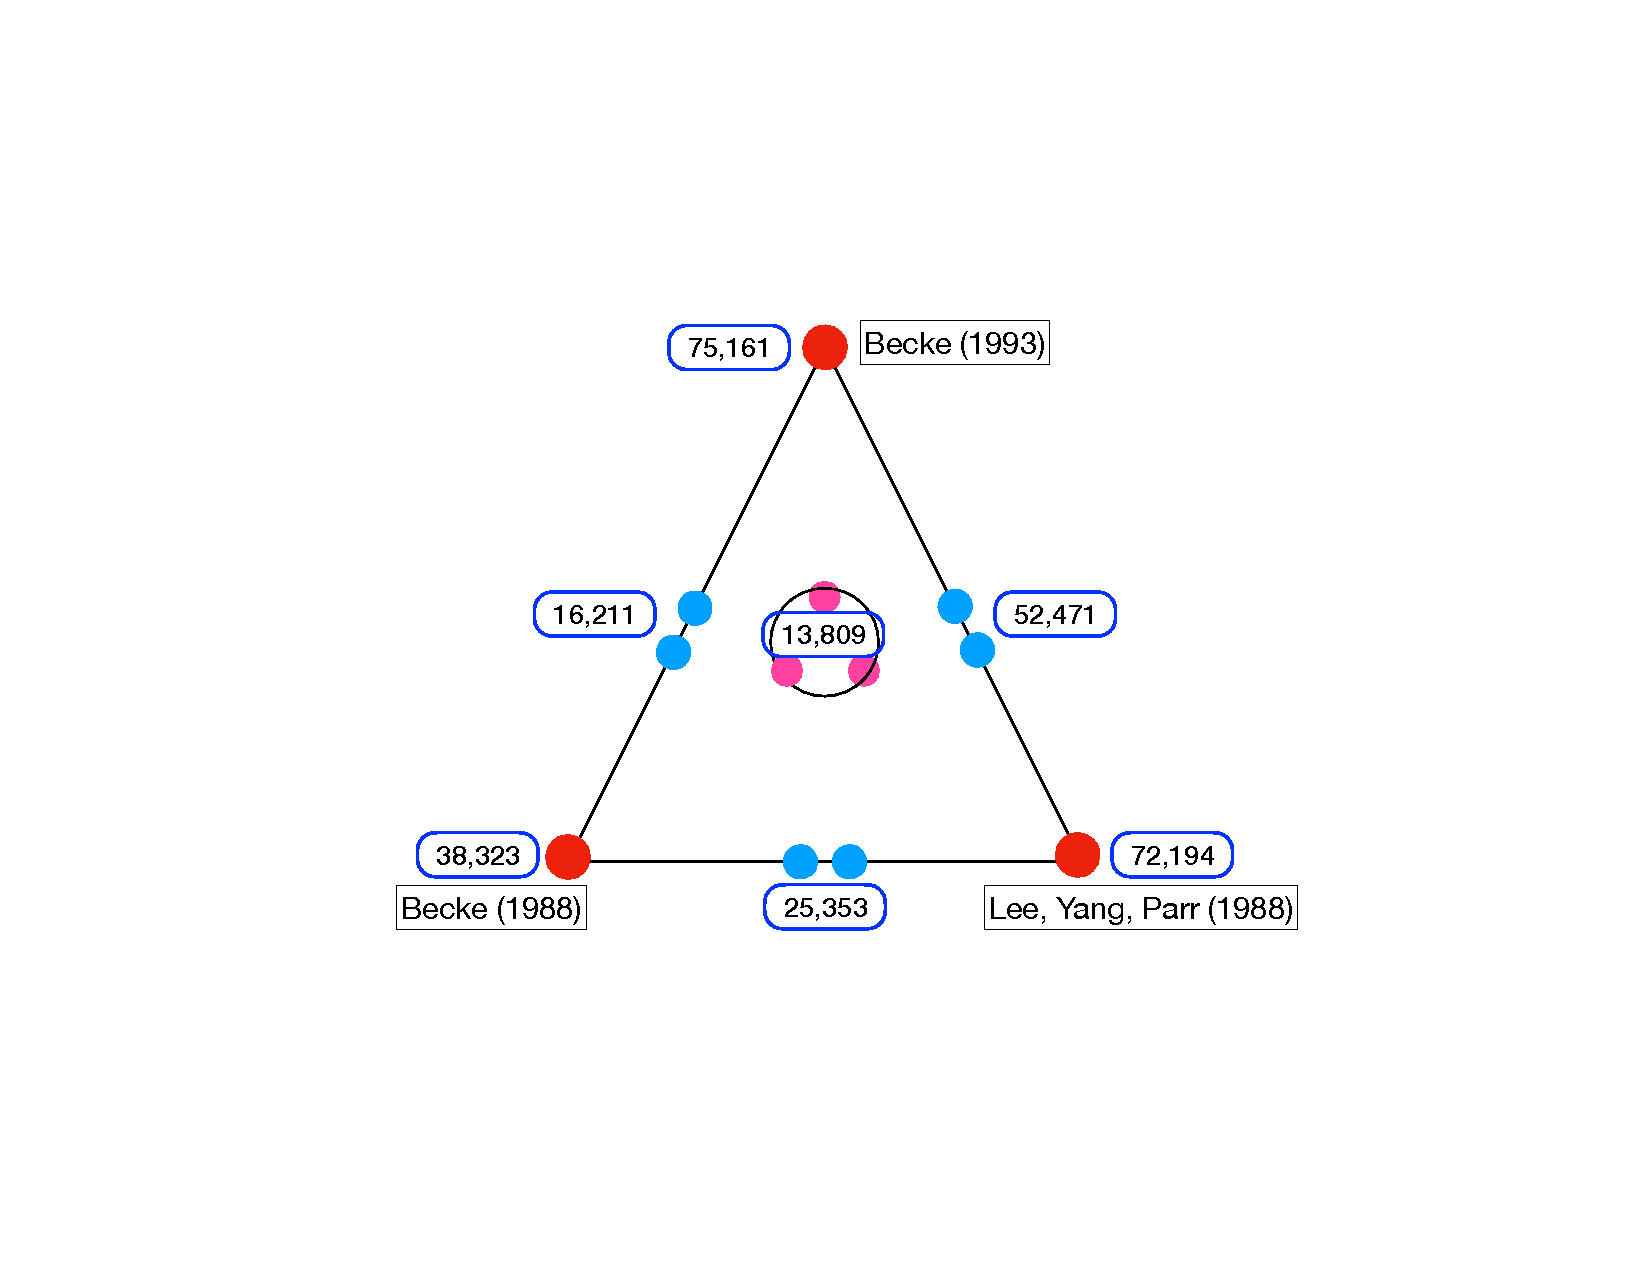
\includegraphics[width=10cm]{fig1.pdf}% This is a *.eps file
\end{center}
\caption{A high frequency triplet. The triad of (i) Becke (1988), (ii) Becke (1992), and (iii) Lee, Yang, and Parr (1988).  Frequencies (round rectangles with blue borders) are shown for the tri-citation (center of triangle), co-citations (sides of triangle), and 
article citations (vertices of triangle). 
}
\label{fig:fig2}
\end{figure}

\end{document}